\documentclass[12pt]{article}
\newif\ifanswer\answertrue%\answerfalse% comment out to show/hide answers
\usepackage{../preamble}% preamble always after \newif\ifanswer
\renewcommand{\theenumi}{\alph{enumi}}
%\pagenumbering{gobble}
\title{Flintridge Prep Summer School, Algebra II \\ June-July 2021}
\author{Patrick \& James Toche}
\date{Revised:~\today}

\begin{document}
\maketitle
\begin{minipage}{\textwidth}
\begin{abstract}\setlength{\parindent}{0pt}%
Notes on the Flintridge Prep Summer Course Algebra II.
Copyright restrictions may apply. Written for personal use. 
Please report typos and errors over at \url{https://github.com/ptoche/Math/tree/master/aops}. 
\end{abstract}
\end{minipage}

\thispagestyle{empty}
\clearpage


%%%%%%%%%%%%%%%%%%%%%%%%%%%%%%%%%%%%%%%%%%%%%%%%%%%%%%%%%%%%%%%%%%%%%%%%
\section{Problem Solving}

\nopagebreak

After summer school is over, M. will go back to her job at the local health-food store, where one of the more challenging tasks she has to do is mixing juices for all the hipster customers who really dig mixed juice. She did a particular mix one day of ginger and apple juice. A cup of ginger juice costs $\$2.65$, and a cup of apple juice costs $\$1.98$. The first customer to come in can only afford to pay $\$18$ for $8$ cups of juice. How many cups of ginger and apple juice should M. use in the mixture, respectively? (round your answers to the nearest tenth of a cup) 

\begin{answer}
Let $A$ denote the quantity of Apple juice and $G$ the quantity of Ginger juice used in the mix (in units of ``cup''). The sum of these must equal $8$ cups. The total cost of the mix must be $\$18$ ($18/8=\$2.25$ per cup of mix). We have a linear system of two equations in two unknowns.
\begin{align*}
 2.65 G + 1.98 A & = 18 \\
           G + A & = 8
\end{align*}
We can solve for $G$ and $A$ by substitution:
\begin{align*}
 2.65 G + 1.98 (8 - G) & = 18 \\
           G & = \frac{18-8 \times 1.98}{2.65-1.98} = \frac{2.16}{0.67} \\
           G & \approx 3.2 \\
           A & \approx 4.8 \\
\end{align*}
\begin{empheq}[box={\mathbox[colback=white]}]{equation*}
    G = 3.2, \quad A = 4.8
\end{empheq} 
\end{answer}
%%%%%%%%%%%%%%%%%%%%%%%%%%%%%%%%%%%%%%%%%%%%%%%%%%%%%%%%%%%%%%%%%%%%%%%%

\iftoggle{showAnswers}{\newpage}


%%%%%%%%%%%%%%%%%%%%%%%%%%%%%%%%%%%%%%%%%%%%%%%%%%%%%%%%%%%%%%%%%%%%%%%%
\section{Cartesian Coordinates}

\nopagebreak

The diagram shows a screen on which the lines $5x+4y=32$ and $-5x+6y=8$ have been graphed. The window settings for this diagram consist of two inequalities, $a\leq x\leq b$ and $c\leq y\leq d$, in which the numbers $a$, $b$, $c$, and $d$ are determined by the diagram. What are these numbers? 
\begin{center}
  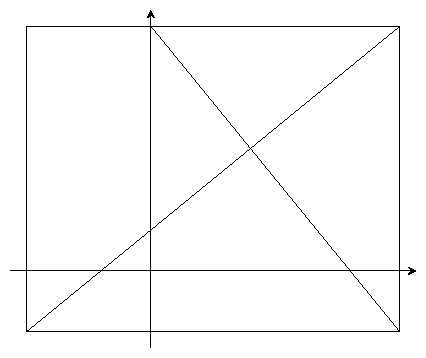
\includegraphics[height=4cm,page=1]{flintprep-problem-02}
\end{center}
\begin{answer}
First, place labels on the figure. 

\begin{center}
  \colorbox{white}{\includegraphics[height=9cm,page=2]{flintprep-problem-02}}
\end{center}

The top-left corner, at the $y$-coordinate $d$, is the intercept of the line with equation $5x+4y=32$. Thus, $d$ is the intercept of the line, and thus $d=8$. The top-right corner has the same $y$-coordinate $8$ and $x$-coordinate $b$ and lies on the line with equation $-5x+6y=8$. Thus the point $(b,8)$ must satisfy the equation, and thus $b=8$. We can go on to solve for all values as follows:
\begin{align*}
(0,d) \in \{5x + 4y = 32\} 
  & \quad\Rightarrow\quad
  5 \cdot 0 + 4 \cdot d = 32
  \quad\Rightarrow\quad
  d = 8 \\
(b,d) = (b,8) \in \{-5x + 6y = 8\} 
  & \quad\Rightarrow\quad
  -5 \cdot b + 6 \cdot 8 = 8
  \quad\Rightarrow\quad
  b = 8 \\  
(b,c) = (8,c) \in \{5x + 4y = 32\} 
  & \quad\Rightarrow\quad
  5 \cdot 8 + 4 \cdot c = 32
  \quad\Rightarrow\quad
  c = -2 \\
(a,c) = (a,-2) \in \{-5x + 6y = 8\} 
  & \quad\Rightarrow\quad
  -5 \cdot a + 6 \cdot (-2) = 8
  \quad\Rightarrow\quad
  a = -4
\end{align*}
\begin{empheq}[box={\mathbox[colback=white]}]{equation*}
    a = -4, \quad b = 8,  \quad c = -2,  \quad d = 8
\end{empheq} 
\end{answer}
%%%%%%%%%%%%%%%%%%%%%%%%%%%%%%%%%%%%%%%%%%%%%%%%%%%%%%%%%%%%%%%%%%%%%%%%

\iftoggle{showAnswers}{\newpage}

%%%%%%%%%%%%%%%%%%%%%%%%%%%%%%%%%%%%%%%%%%%%%%%%%%%%%%%%%%%%%%%%%%%%%%%%
\section{Speed, Distance, Time}

\nopagebreak

A car went a distance of $90$km at a steady speed and returned along the same route at half that speed. The time needed for the whole round trip was four hours and a half. Find the two speeds. 

\begin{answer}
Since  velocity $v$ (speed) is defined over a short distance $d$ and duration $t$ as the ratio $d/t$, if we know both the duration and the constant velocity, we can calculate a distance as $d=vt$. Since the speed is constant over each trip, there are two regimes. Let $v_{1}, t_{1}$ denote velocity/duration for the first part of the trip and $v_{2},t_{2}$ for the second part. We know that $t_{1}+t_{2}=4.5$ hours and $v_{1}=v_{2}/2$. We also have $d_{1}=d_{2}=90$. Thus,
\begin{align*}
        v_{1} & = 2 v_{2} \\
t_{1} + t_{2} & = 4.5 \\
  v_{1} t_{1} & = 90\\
  v_{2} t_{2} & = 90
\end{align*}
This is a linear system of $4$ equations in $4$ unknowns. Eliminate $v_{1},v_{2}$ to get a two-equation system in $t_{1},t_{2}$, from which $v_{1}$ and $v_{2}$ can be recovered:
\begin{align*}
          v_{1} & = 2 v_{2} \\
          v_{2} & = 90/t_{2}\\
2 t_{1} - t_{2} & = 0 \\
  t_{1} + t_{2} & = 4.5
\end{align*}
Solution:
\begin{align*}
        t_{1} = 1.5, \quad
        t_{2} = 3,   \quad
        v_{1} = 60,  \quad
        v_{2} = 30
\end{align*}
\begin{empheq}[box={\mathbox[colback=white]}]{equation*}
        v_{1} = 60,\quad v_{2} = 30
\end{empheq} 
\end{answer}
%%%%%%%%%%%%%%%%%%%%%%%%%%%%%%%%%%%%%%%%%%%%%%%%%%%%%%%%%%%%%%%%%%%%%%%%

\iftoggle{showAnswers}{\newpage}

%%%%%%%%%%%%%%%%%%%%%%%%%%%%%%%%%%%%%%%%%%%%%%%%%%%%%%%%%%%%%%%%%%%%%%%%
\section{Problem 293}

\nopagebreak

The Prep Ski club is planning a trip to Mammoth during semester break. They have $40$ skiers signed up to go, and the ski resort is charging $\$120$ for each person. 

\begin{enumerate}

\item 
Calculate how much money (revenue) the resort expects to take in.

\begin{answer}
\begin{align*}
40 \times \$120 = \$ 4800
\end{align*}
\end{answer}

\item 
The resort manager offers to reduce the group rate of $\$120$ per person by $\$2$ for each additional registrant, as long as the revenue continues to increase. For example, if $5$ more skiers sign up, all $45$ would pay $\$110$ each, producing revenue of $\$4950$ for the resort. Fill in the table for the manager. 

\begin{center}
\renewcommand{\arraystretch}{1.5}
\newcolumntype{C}[1]{>{\centering\arraybackslash}p{#1}} % centered 'p' col.
\begin{tabular}{*{4}{C{0.2\linewidth}}}
    \hline
    extras & persons & cost/person & revenue \\
    \hline
    $0$    &   $40$  &         &  \\
    $1$    &   $41$  &         &  \\
    $2$    &   $42$  &         &  \\
    $3$    &   $43$  &         &  \\
    $4$    &   $44$  &         &  \\
    $5$    &   $45$  &  $110$  & $4950$\\
    $6$    &   $46$  &         &  \\
    $7$    &   $47$  &         &  \\
    $8$    &   $48$  &         &  \\
    $9$    &   $49$  &         &  \\
    $10$   &   $50$  &         &  \\
    $11$   &   $51$  &         &  \\
    $12$   &   $52$  &         &  \\
    \hline
    \end{tabular}
\end{center}


\begin{answer}
\begin{center}
\renewcommand{\arraystretch}{1.5}
\newcolumntype{C}[1]{>{\centering\arraybackslash}p{#1}} % centered 'p' col.
\begin{tabular}{*{4}{C{0.2\linewidth}}}
    \hline
    extras & persons & cost/person & revenue \\
    \hline
    $0$    &   $40$  &   $120$  &   $4800$\\
    $1$    &   $41$  &   $118$  &   $4838$\\
    $2$    &   $42$  &   $116$  &   $4872$\\
    $3$    &   $43$  &   $114$  &   $4902$\\
    $4$    &   $44$  &   $112$  &   $4928$\\
    $5$    &   $45$  &   $110$  &   $4950$\\
    $6$    &   $46$  &   $108$  &   $4968$\\
    $7$    &   $47$  &   $106$  &   $4982$\\
    $8$    &   $48$  &   $104$  &   $4992$\\
    $9$    &   $49$  &   $102$  &   $4998$\\
    $10$   &   $50$  &   $100$  &   $5000$\\
    $11$   &   $51$  &    $98$  &   $4998$\\
    $12$   &   $52$  &    $96$  &   $4992$\\
    \hline
    \end{tabular}
\end{center}

\end{answer}

\item 
Let $x$ be the number of new registrants. In terms of $x$, write expressions for the total number of persons going, the cost to each, and the resulting revenue for the resort.

\begin{answer}
\begin{align*}
\text{number of persons} &: 40 + x\\
\text{cost per person} &: 120 - 2x\\
\text{total revenue} &: (120 - 2x) (40 + x)
\end{align*}
\end{answer}

\item 
Plot your revenue values versus $x$, for the relevant values of $x$. Because this is a discrete problem, it does not make sense to connect the dots. 

\begin{answer}
Revenue is a quadratic function of the number of new registrants $x$.
\begin{align*}
(120 - 2x) (40 + x) 
& = - 2x^2 + 40x + 4800 \\
& = - 2 (x^2 - 20x - 2400) \\
& = - 2 ((x - 10)^2 - 100 - 2400) \\
& = - 2 ((x - 10)^2 - 50^2) \\
& = - 2 (x - 10 - 50)(x - 10 + 50) \\
& = - 2 (x - 60)(x + 40) 
\end{align*}
Revenue starts at $40 \times \$120 = \$4800$ for $x=0$, rises then falls to $0$ for $x=60$. 

\begin{center}
  \colorbox{white}{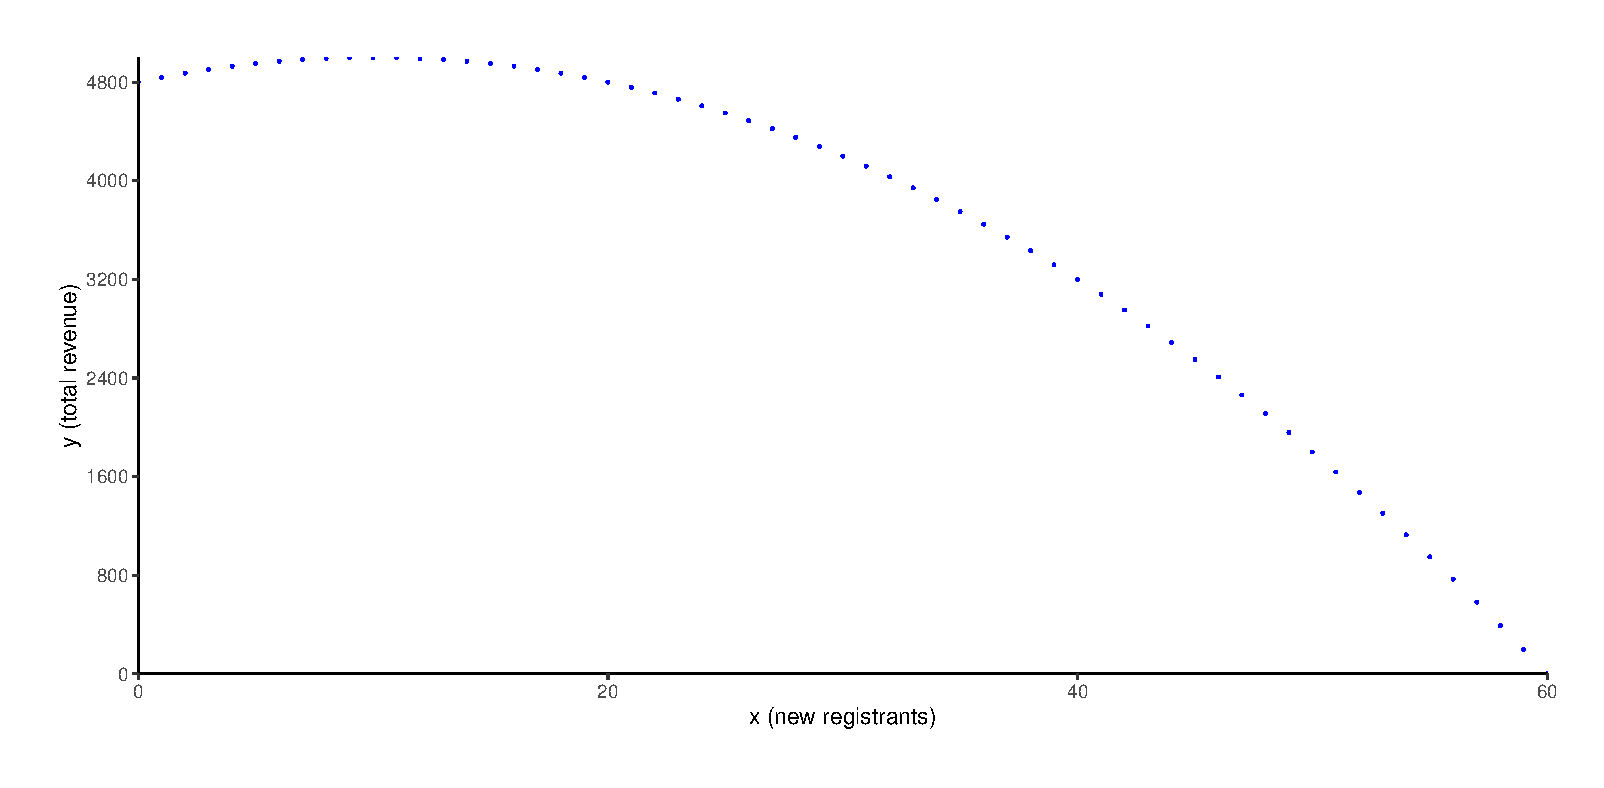
\includegraphics[width=0.95\linewidth]{flintprep-293}}
\end{center}

To see the big picture, we plot revenue in terms of the total number of registrants: Revenue starts at $0$, rises to a maximum for $50$ registrants, then falls to $0$ for $100$ registrants. 
\begin{center}
  \colorbox{white}{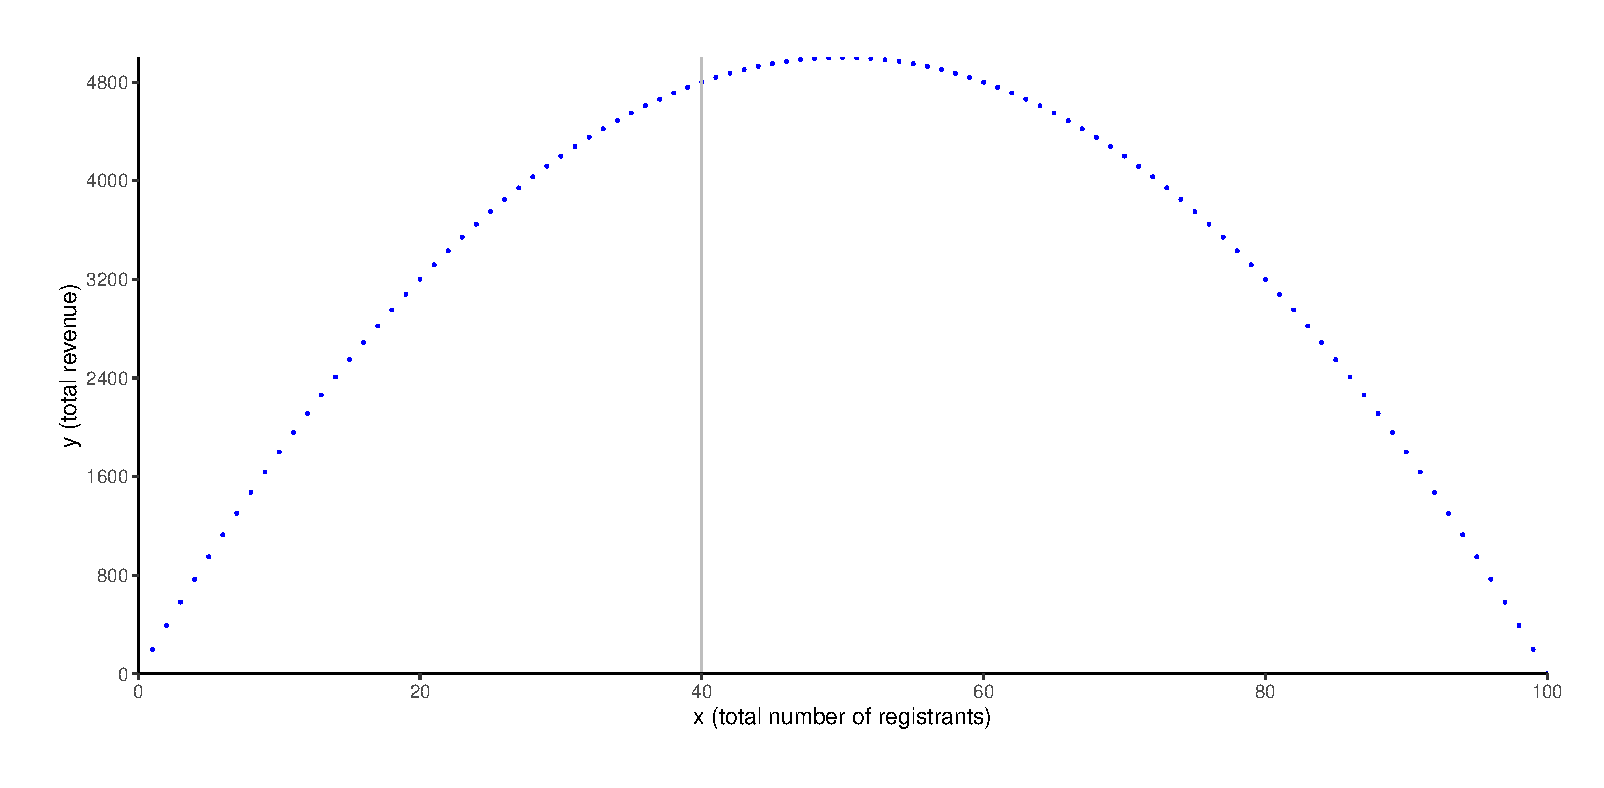
\includegraphics[width=0.95\linewidth]{flintprep-293-total}}
\end{center}
\end{answer}

\item 
For the resort to take in at least $\$4900$, how many skiers must go on the trip?

\begin{answer}
The condition on revenue is:
\begin{align*}
y = (120 - 2x) (40 + x) & \geq 4900
\end{align*}
Solve for $x$ when the inequality is strict:
\begin{align*}
    (120 - 2x) (40 + x) & = 4900 \\
          -2 x^2 + 40 x & = 100 \\
             x^2 - 20 x & = -50 \\
        (x-10)^2 - 10^2 & = -50 \\
     (x-10-\sqrt{50})(x-10+\sqrt{50}) & = 0
\end{align*}
The roots are approximately $17.07$ and $2.92$. The closest integers associated with revenue greater than $4900$ are $x=17$ and $x=3$. The corresponding revenues are:
\begin{align*}
x = 3:  & y = (120 - 2 \cdot 3) (40 + 3) = 4902 \\
x = 17: & y = (120 - 2 \cdot 17) (40 + 17) = 4902
\end{align*}
Any value in between generates even greater revenue. Thus, the resort can take in any number of new registrants between $3$ and $17$ or, equivalently, a total number skiers between $43$ and $57$. The maximal revenue is achieved for $x=10$ new registrants, or $50$ skiers, with a revenue of $y=\$5000$.
\end{answer}

\iftoggle{showAnswers}{\newpage}

%%%%%%%%%%%%%%%%%%%%%%%%%%%%%%%%%%%%%%%%%%%%%%%%%%%%%%%%%%%%%%%%%%%%%%%%
\section{Question 11 of MidTerm Test}

\nopagebreak

After high school, N. gets a job at the fire department, and is in charge of operating the hose, which shoots water out in a parabolic arc. Assume the behavior of the hose can be modeled by quadratic function. The hose is sprayed from $4.5$ feet above ground, and hits the ground a horizontal distance of $58$ feet away. The maximum height of the water occurs $28$ feet from where the hose is sprayed. Let $x$ bet the horizontal distance from the hose nozzle, and $y$ be the corresponding height of the stream of water, both in feet. 

\begin{enumerate}

\item What is the quadratic equation that models the path of the water?

\begin{answer}
One of the roots is at $x=58$. Since the maximum height occurs at $28$ feet, the vertex is located at $x=28$. This gives the second root as $x=58-2\times(58-28)=-2$. This gives a quadratic equation of the form:
\begin{align*}
y = a(x+2)(x-58)
\end{align*}
where $a$ is determined as follows. The $y$ intercept is at $4.5$ feet, so
\begin{align*}
4.5 = a(0+2)(0-58) 
\quad\Rightarrow\quad
a = -\frac{9}{232} \approx 0.0043
\end{align*}
Obviously $a<0$ since the path of the water is up then down. 
\end{answer}

\item Graph the function.

\begin{answer}
\begin{center}
  \colorbox{white}{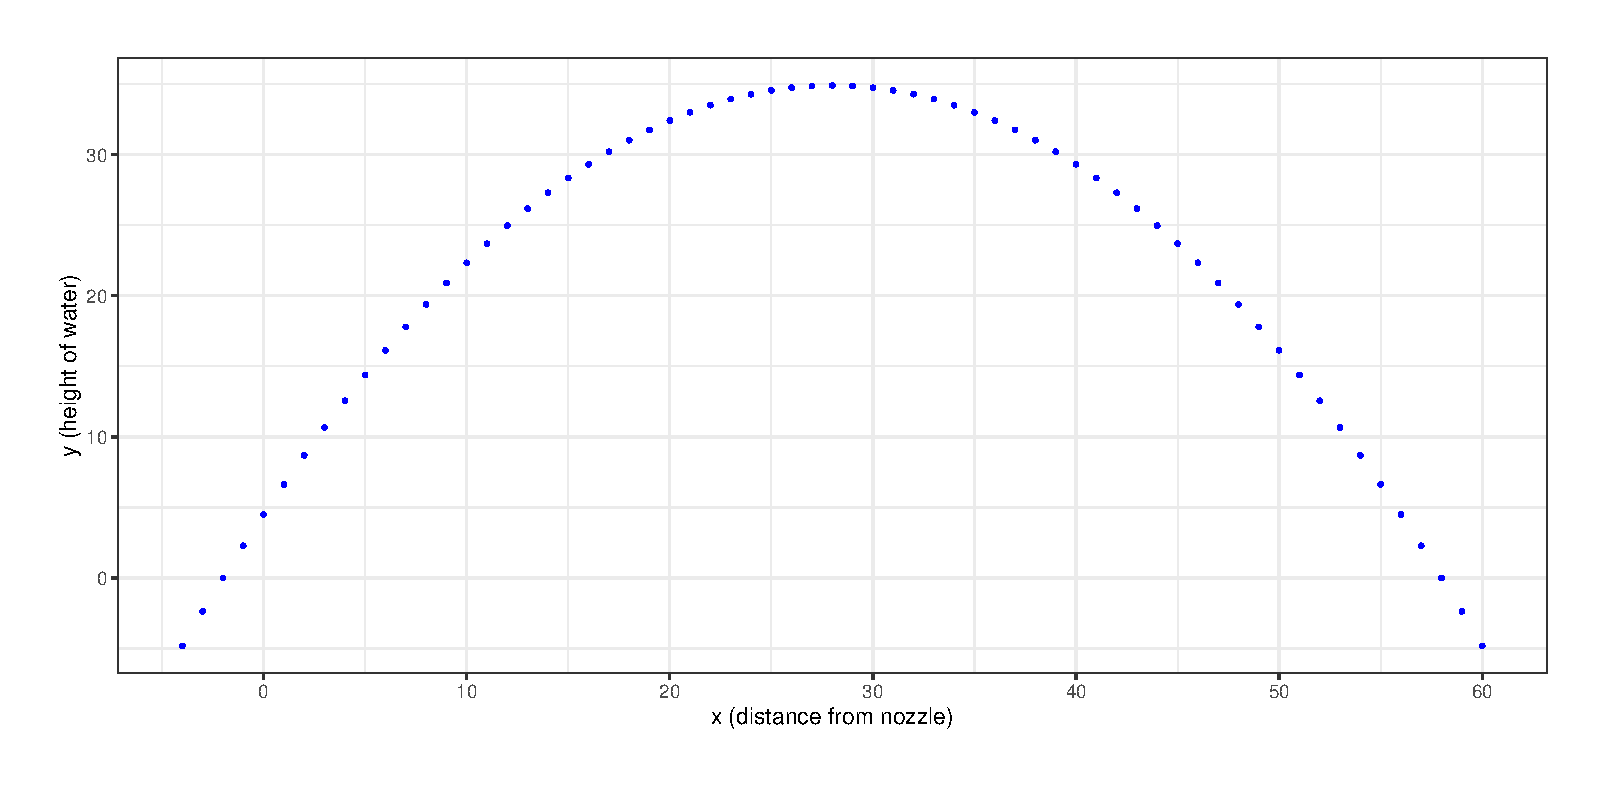
\includegraphics[width=0.95\linewidth]{flintprep-midterm-11}}
\end{center}
\end{answer}

\item What is the maximum height of the water?

\begin{answer}
The maximum height occurs for $x=28$:
\begin{align*}
y = -\frac{9}{232} \, (28+2)(28-58) 
  = \frac{9 \times 30^2}{232}
  = \frac{2025}{58} 
  \approx 34.9
\end{align*} 
\end{answer}

\item Will the stream go over a $6$ ft high fence that is located $48$ feet from the nozzle? Explain your reasoning and show any work that is needed. 

\begin{answer}
The question is whether $y>6$ for $x=48$:
\begin{align*}
y = -\frac{9}{232} \, (48+2)(48-58) 
  = \frac{1125}{58}
  \approx 19.4
\end{align*} 
The height of the water is more than three times greater than the fence. 
\end{answer}

\end{enumerate}
%%%%%%%%%%%%%%%%%%%%%%%%%%%%%%%%%%%%%%%%%%%%%%%%%%%%%%%%%%%%%%%%%%%%%%%%

\iftoggle{showAnswers}{\newpage}

%%%%%%%%%%%%%%%%%%%%%%%%%%%%%%%%%%%%%%%%%%%%%%%%%%%%%%%%%%%%%%%%%%%%%%%%
\section*{The Shortest Fence}

\nopagebreak

A fence that is $9$ feet tall is situated $8$ feet from the side of a wall. A ladder is leaning against the wall, with its base outside the fence, just touching the top of the fence. The ladder is leaning at an angle of $t$ degrees relative to the ground. Find the length of the ladder. Find the length of the shortest ladder that could reach the building from outside the fence. 

\begin{answer}
\begin{center}
  \colorbox{white}{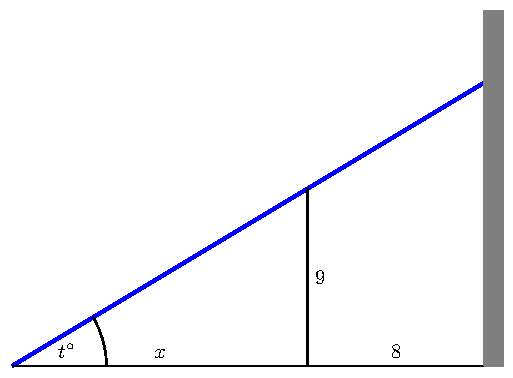
\includegraphics[height=6cm,page=1]{flintprep-problem-514}}
\end{center}

The line traced by the ladder is colored blue. The wall against which the ladder rests is colored gray. The distance marked $x$ is missing. Note that the ladder does not reach to the top of the wall. 

Recall the following rules of trigonometry:
\begin{align*}
\sin(t) & = \frac{\text{opposite}}{\text{hypotenuse}} \\
\cos(t) & = \frac{\text{adjacent}}{\text{hypotenuse}} \\
\tan(t) & = \frac{\text{opposite}}{\text{adjacent}}
\end{align*}

Since we know the angle and the length of the opposite leg of the short triangle, we can find $x$ from the tangent formula:
\begin{align*}
\tan(t) & = \frac{9}{x} 
\quad\Rightarrow\quad
x = \frac{9}{\tan(t)}
\end{align*}

Since the leg of the large triangle is $x+8$, we can now find the length of the ladder $l$ -- the hypotenuse of the large triangle -- from the cosine formula:
\begin{align*}
\cos(t) & = \frac{x+8}{l} 
\quad\Rightarrow\quad
l = \frac{x+8}{\cos(t)}
\end{align*}

Substituting the value of $x$ found earlier yields
\begin{align*}
l = \frac{\frac{9}{\tan(t)}+8}{\cos(t)} 
  = \frac{8}{\cos(t)} + \frac{9}{\cos(t)\tan(t)}
\end{align*}
But by definition $\cos(t)\tan(t)=\sin(t)$, so the expression simplifies to:
\begin{empheq}[box={\mathbox[colback=white]}]{equation*}
l = \frac{8}{\cos(t)} + \frac{9}{\sin(t)}
\end{empheq}

The shortest ladder is the one that minimizes the length of the hypotenuse. Thus, we select $t$ to minimize the length of the hypotenuse:
\begin{align*}
\frac{8}{\cos(t)} + \frac{9}{\sin(t)}
\end{align*}

If we knew calculus, we would set the derivative of this expression to zero. To compute the derivative, we need the following differentiation rules:
\begin{align*}
\frac{d}{dt} \frac{1}{f(t)} 
  & = \frac{-\frac{d}{dt}f(t)}{f^2(t)} \\
\frac{d}{dt} \cos(t)
  & = -\sin(t) \\
\frac{d}{dt} \sin(t)
  & = +\cos(t) 
\end{align*}
Combining these two facts yields:
\begin{align*}
\frac{d}{dt} \frac{1}{\cos(t)} 
  & = \frac{\sin(t)}{\cos^2(t)} \\
\frac{d}{dt} \frac{1}{\sin(t)} 
  & = \frac{-\cos(t)}{\sin^2(t)} 
\end{align*}

We can now differentiate $l(t)$ with respect to $t$:
\begin{align*}
\frac{d}{dt} l(t) 
  = 
  \frac{8\sin(t)}{\cos^2(t)} 
  - \frac{9\cos(t)}{\sin^2(t)} 
  = 
  \frac{8\sin^{3}(t) - 9\cos^{3}(t)}{\cos^2(t)\sin^2(t)} 
\end{align*}
And thus 
\begin{align*}
\frac{d}{dt} l(t) = 0
\quad\Rightarrow\quad
   8\sin^{3}(t) & = 9\cos^{3}(t) \\
    \tan^{3}(t) & = \frac{9}{8} \\[1ex]
        \tan(t) & = \frac{\sqrt[3]{9}}{2} 
                  \approx 1.04 
                  \quad\Rightarrow\quad
                t \approx 46.12^{\circ} 
\end{align*}

In general, if the distance to the wall is $d$ and the height of the fence $h$, the shortest ladder has a tangent equal to:
\begin{empheq}[box={\mathbox[colback=white]}]{equation*}
  \tan(t) = \sqrt[3]{h/d}
\end{empheq} 

\end{answer}
%%%%%%%%%%%%%%%%%%%%%%%%%%%%%%%%%%%%%%%%%%%%%%%%%%%%%%%%%%%%%%%%%%%%%%%%

\iftoggle{showAnswers}{\newpage}

%%%%%%%%%%%%%%%%%%%%%%%%%%%%%%%%%%%%%%%%%%%%%%%%%%%%%%%%%%%%%%%%%%%%%%%%
\section{A Bouncing Ball}

\nopagebreak

A ball is dropped from a height of $h$ feet and left to bounce forever. The rebound ratio of the ball is $r$. The time required to fall from a height of $h$ feet (or to rise to that height after a bounce) is $\sqrt{h}/4$ seconds.  Find a formula for the total distance traveled by the ball, and for the total time needed to cover that distance. 

\begin{answer}
Let $n$ denote the index associated with a point of contact with the ground. At index $0$, the ball makes the first contact with the ground, after dropping from height $h$. At index $1$, the ball makes the second contact, after rising to height $rh$ and dropping all the way back. With this notation, the ball has bounced $n$ times at index $n-1$. 

Let $a_{n}$ denote the heights starting from index $1$, in other words not including the initial drop from height $h$, and let $s_{n}$ denote the sum of the heights of $n$ bounces, that is
\begin{align*}
s_{n} = \sum_{k=1}^{k=n} a_{k}
\end{align*}
where the height of the bounces are given by
\begin{align*}
a_{k} & = a_{1} r^{k-1} \\
a_{1} & = hr
\end{align*}

Let $d_{n}$ denote the total distance traveled by the ball after $n$ bounces. We have:
\begin{align*}
d_{n} = h + 2s_{n-1}
\end{align*}
Here the first bounce is associated with index $0$, the second bounce with index $1$, etc..
\begin{align*}
s_{n} 
  = \sum_{k=1}^{k=n} a_{k}
  = a_{1} \sum_{k=1}^{k=n} r^{k-1} 
  = a_{1} \frac{1-r^{n}}{1-r} 
  = hr \frac{1-r^{n}}{1-r} 
\end{align*}
Substitute $s_{n-1}$ back into $d_{n}$ yields:
\begin{empheq}[box={\mathbox[colback=white]}]{equation*}
  d_{n} = h + 2hr \frac{1-r^{n-1}}{1-r}
\end{empheq} 

For an infinite number of bounces, let $n\rightarrow\infty$,
\begin{align*}
d_{n} \longrightarrow h + \frac{2hr}{1-r}
\quad\text{as}\quad n\longrightarrow\infty
\end{align*}
and the time it takes to bounce infinitely many times is:
\begin{align*}
\frac{1}{4} \, \sqrt{h + 2hr/(1-r)}
\end{align*}

While the total number of bounces is infinite, the distance traveled by the ball is finite and it stops bouncing in finite time. 
\end{answer}
%%%%%%%%%%%%%%%%%%%%%%%%%%%%%%%%%%%%%%%%%%%%%%%%%%%%%%%%%%%%%%%%%%%%%%%%

\iftoggle{showAnswers}{\newpage}

%%%%%%%%%%%%%%%%%%%%%%%%%%%%%%%%%%%%%%%%%%%%%%%%%%%%%%%%%%%%%%%%%%%%%%%%
\section{Loan Repayment}

\nopagebreak

Let $A_{0}$ be a loan to be repaid in full after $t$ payments. Let $A_{n}$ be the amount owed after $n$ payments. The bank charges a monthly interest on the outstanding balance at rate $r$. The loan contract states that a (constant) monthly payment $P$ is due until full repayment. The first payment is due at the end of the first month. Express $A_{n}$ in terms of $A_{n-1}$. Express $A_{n}$ in terms of $A_{0}$. Solve for the constant payment $P$ that achieves a full repayment after $t$ years. 

\begin{answer}
The monthly recursion is
\begin{align*}
A_{n} = (1+r) A_{n-1} - P
\end{align*}

This is an algebraic series, which may be solved in terms of $A_{0}$ by repeated substitution:
\begin{align*}
A_{n} 
  & = (1+r) A_{n-1} - P \\
  & = (1+r) [(1+r) A_{n-2} - P] - P \\
  & = (1+r)^{2} A_{n-2} - (1+r) P - P \\
  & = (1+r)^{k} A_{n-k} - (1+r)^{k-1} P -\ldots -(1+r)^{1} P - (1+r)^{0} P \\
\text{set $k=n$:}  \qquad\quad
  & = (1+r)^{n} A_{0} - (1+r)^{n-1} P -\ldots -(1+r)^{1} P - (1+r)^{0} P \\
  & = (1+r)^{n} A_{0} - P \, [1 + (1+r) + \ldots + (1+r)^{n-1}] \\[1ex]
  & = (1+r)^{n} A_{0} - P \, \frac{(1+r)^{n}-1}{(1+r)-1}
\end{align*}
The balance after $t$ payments is:
\begin{empheq}[box={\mathbox[colback=white]}]{equation*}
A_{t} = (1+r)^{t} A_{0} - P \, \frac{(1+r)^{t}-1}{r} 
\end{empheq} 

To see that the formula is correct, check the first few cases:
\begin{align*}
A_{1} 
  & = (1+r)^{1} A_{0} - P \, \frac{(1+r)^{1}-1}{r} 
    = (1+r) A_{0} - P \qquad\cmark \\
A_{2} 
  & = (1+r)^{2} A_{0} - P \, \frac{(1+r)^{2}-1}{r} \\
  & = (1+r)^{2} A_{0} - P \, \frac{r^{2}+2r}{r} \\
  & = (1+r)^{2} A_{0} - P(1+r) - P \qquad\cmark 
\end{align*}

Full repayment is achieved for $P$ such that $A_{t}=0$,
\begin{align*}
(1+r)^{t} A_{0} 
  & = P \, \frac{(1+r)^{t}-1}{r} \\[1ex]
P 
  & = \frac{(1+r)^{t}}{(1+r)^{t}-1} \, rA_{0} \\[1ex]
  & = rA_{0} + \frac{rA_{0}}{(1+r)^{t}-1} 
\end{align*}
Note that for a perpetual loan, as $t\rightarrow\infty$, the perpetuity payment is simply:
\begin{align*}
P \longrightarrow rA_{0} \quad\text{as}\quad t\longrightarrow\infty
\end{align*}
\end{answer}
%%%%%%%%%%%%%%%%%%%%%%%%%%%%%%%%%%%%%%%%%%%%%%%%%%%%%%%%%%%%%%%%%%%%%%%%

\iftoggle{showAnswers}{\newpage}

%%%%%%%%%%%%%%%%%%%%%%%%%%%%%%%%%%%%%%%%%%%%%%%%%%%%%%%%%%%%%%%%%%%%%%%%
\section{Present Value Calculation}

\nopagebreak

An NBA center recently signed a seven-year contract for $\$121$ million. What is the present value of this contract, given a $9\%$ interest rate?

\begin{answer}
Let $r$ denote the interest rate on the bank balance, $r=0.09$. Let $P$ denote the annual payment, 
\begin{align*}
P = \frac{121,000,000}{7}
\end{align*}
The present discounted value of the seven payments is:
\begin{align*}
\text{Present Value}~ =
P + \frac{P}{1+r} + \frac{P}{(1+r)^2} + \ldots + \frac{P}{(1+r)^6}
\end{align*}
To clarify the derivation, let $a =\dfrac{1}{1+r}$. 
\begin{align*}
\text{Present Value}~ =
P \, (1 + a + a^2 + \ldots + a^6)
 & = P \cdot \frac{1-a^7}{1-a}
\end{align*}
Substituting $r$ back into the expression,
\begin{align*}
\text{Present Value}~
 & = P \cdot \frac{1-\left(\frac{1}{1+r}\right)^7}{1-\frac{1}{1+r}} \\
 & = P \cdot \frac{(1+r)^7-1}{(1+r)^7} \cdot \frac{1+r}{r} \\
 & = P \cdot \frac{(1+r)^7-1}{r(1+r)^6} \\
 & = \frac{121,000,000}{7} \cdot \frac{(1.09)^7-1}{0.09(1.09)^6} \\
 & \approx 94,828,021
\end{align*}
%% 121000000/7 * ((1.09)^7-1) / 0.09 / (1.09)^6 
%% 94828021
\begin{empheq}[box={\mathbox[colback=white]}]{equation*}
 \text{Present Value}~ \approx 94,828,021
\end{empheq} 
\end{answer}
%%%%%%%%%%%%%%%%%%%%%%%%%%%%%%%%%%%%%%%%%%%%%%%%%%%%%%%%%%%%%%%%%%%%%%%%

\iftoggle{showAnswers}{\newpage}

%%%%%%%%%%%%%%%%%%%%%%%%%%%%%%%%%%%%%%%%%%%%%%%%%%%%%%%%%%%%%%%%%%%%%%%%
\section{Contract Valuation}

\nopagebreak

An NBA center recently signed a seven-year contract for $\$121$ million. How much must the club invest when the contract is signed, so that it can make seven equal payments, the first one due immediately, given a $9\%$ interest rate? 

\begin{answer}
Let $r$ denote the interest rate on the bank balance, $r=0.09$. Let $P$ denote the annual payment, 
\begin{align*}
P = \frac{121,000,000}{7}
\end{align*}
Let $B_{t}$ denote the cash balance at the start of period $t$. The bank balance evolves as:
\begin{align*}
t & = 1 \qquad B_{1} = I - P\\
t & = 2 \qquad B_{2} = (1+r)B_{1} - P\\
  &\vdotswithin{=} \\
t & = n \qquad B_{n} = (1+r)B_{n-1} - P
\end{align*}
The initial investment $I$ and the first payment $P$ occur at the \underline{start} of the contract ($t=1$). The initial balance $B_{1}$ is immediately placed in an interest-paying account. By the \underline{start} of the second year, the balance has grown to $(1+r)B_{1}$, and the second payment $P$ is made. The process continues until the seventh payment is completed.

Note! In some problems the first payment and accrued interest occur simultaneously at the end of the first period, but here the first payment is due one period before the interest accrues. The difference is that $B_{1}$ would be $I$ instead of $I-P$. 

To express the final balance $B_{n}$ in terms of the initial investment $I$, we repeatedly substitute, rearrange, and deduce the general pattern:
\begin{align*}
B_{n} & = (1+r)B_{n-1} - P\\
      & = (1+r)(\, (1+r)B_{n-2} - P \,) - P\\
      & = (1+r)(\,(1+r)(\,(1+r)B_{n-3} - P \,) - P \,) - P\\
      &\vdotswithin{=}\\
      & = (1+r)^{k}B_{n-k} - (1+r)^{k-1}P - \ldots  - (1+r)P - P
\end{align*}
The formula, returns the same expressions calculated earlier for e.g. $n=1,2$. 

The payments part of the formula can be simplified by recognizing that the $(1+r)^{k}P$ terms form a geometric sum:
\begin{align*}
B_{n} & = (1+r)^{k}B_{n-k} - (1+r)^{k-1}P - \ldots  - (1+r)P - P \\
      & = (1+r)^{k}B_{n-k} - (\, (1+r)^{k-1} + \ldots  + (1+r) +1 \,)  \, P \\
      & = (1+r)^{k}B_{n-k} - \frac{(1+r)^{k}-1}{(1+r)-1\hfill}  \, P \\
      & = (1+r)^{k}B_{n-k} - \frac{(1+r)^{k}-1}{r}  \, P
\end{align*}
Set $k=n-1$
\begin{align*}
B_{n} = (1+r)^{n-1}B_{1} - \frac{(1+r)^{n-1}-1}{r} \, P
\end{align*}
Thus, the balance after $n$ payments, expressed in terms of the initial investment $I$, is
\begin{align*}
B_{n} = (1+r)^{n-1}(I - P) - \frac{(1+r)^{n-1}-1}{r} \, P
\end{align*}

In the special case $n=7$ (seven payments), we get the final balance:
\begin{align*}
B_{7} = (1+r)^{6}(I-P) - \frac{(1+r)^{6}-1}{r} \, P
\end{align*}
The first term includes the first payment, while the second term includes the effect of the next $6$ payments. 

To cover the contract, the club should invest exactly enough to cover the seven payments, so that the balance should be zero after the seventh payment, $B_{7}=0$, implying
\begin{align*}
(1+r)^{6} (I-P)
     & = \frac{(1+r)^{6}-1}{r}  \, P \\
   I & = P + \frac{1-(1+r)^{-6}}{r} \, P
\end{align*}
Plug in the data into the Initial Investment $I$,
\begin{align*}
I & = \frac{121,000,000}{7} \left(1 + \frac{1-(1.09)^{-6}}{0.09} \right) \\
  & \approx 94,828,021
\end{align*}
%% (121000000/7) * (1 + (1-(1.09)^(-6))/0.09)
%% 94828021
The $121$ million dollar contrat can be financed with a little less than $95$ million dollars. That means the bank balances return a total of about $\$26,171,979$ in interest payments over the seven-year period. But note that the initial investment needed to honor the contract is equal to the present value of $121$ million dollars divided into seven annual payments! A simpler approach that yields the same answer is therefore:
\begin{align*}
I = P \cdot \frac{1-a^7}{1-a}
      \qquad \text{where}~ a =\dfrac{1}{1+r}
\end{align*}

\begin{empheq}[box={\mathbox[colback=white]}]{equation*}
    \text{Initial Investment}~ =
    \text{Present Value}~ \approx ~ \$ 94,828,021
\end{empheq}
\end{answer}
%%%%%%%%%%%%%%%%%%%%%%%%%%%%%%%%%%%%%%%%%%%%%%%%%%%%%%%%%%%%%%%%%%%%%%%%

\end{enumerate}
%%%%%%%%%%%%%%%%%%%%%%%%%%%%%%%%%%%%%%%%%%%%%%%%%%%%%%%%%%%%%%%%%%%%%%%%

\iftoggle{showAnswers}{\newpage}

%%%%%%%%%%%%%%%%%%%%%%%%%%%%%%%%%%%%%%%%%%%%%%%%%%%%%%%%%%%%%%%%%%%%%%%%
\section{Algebraic Series}

\nopagebreak

Let $a_{n}$ denote the $n$th term in the algebraic sequence with common difference $d$, and let $s_{n}$ denote the sum of the first $n$ terms, starting with $a_{1}$. Express $s_{n}$ in terms of $a_{1}$, $d$, and $n$. Express $s_{n}$ in terms of $a_{n}$, $d$, and $n$. Express $s_{n}$ in terms of $a_{1}$, $a_{n}$, and $n$ (no $d$).  

\begin{answer}
The algebraic sequence $a_{m}$ satisfies the recursion
\begin{align*}
a_{m} = a_{m-1} + d
\end{align*}
By repeated substitution (at the last step, substitute $k=m-1$),
\begin{align*}
a_{m} & = a_{m-1} + d \\
      & = a_{m-2} + 2d \\
      & = a_{m-k} + kd \\
      & = a_{1} + (m-1)d 
\end{align*}

The algebraic sequence $a_{m}$ also satisfies the recursion
\begin{align*}
a_{m} = a_{m+1} - d
\end{align*}
By repeated substitution (at the last step, substitute $k=n-m$),
\begin{align*}
a_{m} & = a_{m+1} - d \\
      & = a_{m+2} - 2d \\
      & = a_{m+k} - kd \\
      & = a_{n} - (n-m)d 
\end{align*}

We have written the sequence in two ways, which we can use to obtain a third expression:
\begin{align*}
a_{m} & = \frac{1}{2} (a_{1} + (m-1)d) + \frac{1}{2} (a_{n} - (n-m)d) \\
      & = \frac{a_{1} + a_{n}}{2} + \frac{d}{2} (2m-1-n) \\
\quad\Rightarrow\quad
a_{n} & = \frac{a_{1} + a_{n}}{2} + \frac{d(n-1)}{2} 
\end{align*}
The arithmetic sum series is then
\begin{align*}
& s_{n} = \sum_{m=1}^{m=n} a_{m} 
  = \sum_{m=1}^{m=n}\frac{a_{1} + a_{n}}{2} + \frac{d}{2}\sum_{m=1}^{m=n} (2m-1-n)
  = \frac{n(a_{1} + a_{n})}{2} \\
& \text{where}\quad \sum_{m=1}^{m=n} (2m-1-n) 
  = (1-n) + (3-n) + \ldots + (n-3) + (n-1)
  = 0
\end{align*}

\begin{empheq}[box={\mathbox[colback=white]}]{equation*}
a_{m} = \frac{a_{1} + a_{n}}{2}
\qquad 
s_{n} = \frac{n(a_{1} + a_{n})}{2}
\end{empheq} 

\end{answer}
%%%%%%%%%%%%%%%%%%%%%%%%%%%%%%%%%%%%%%%%%%%%%%%%%%%%%%%%%%%%%%%%%%%%%%%%

\iftoggle{showAnswers}{\newpage}

%%%%%%%%%%%%%%%%%%%%%%%%%%%%%%%%%%%%%%%%%%%%%%%%%%%%%%%%%%%%%%%%%%%%%%%%
\section{Trigonometry}

\nopagebreak

Calculate the angles of a triangle with side lengths $5$, $6$, $9$. Calculate its area. 

\begin{answer}
Refer to the figure. Let $a$, $b$, $c$ denote the side lengths and $\alpha$, $\beta$, $\gamma$ the angles. 
\begin{center}
  \colorbox{white}{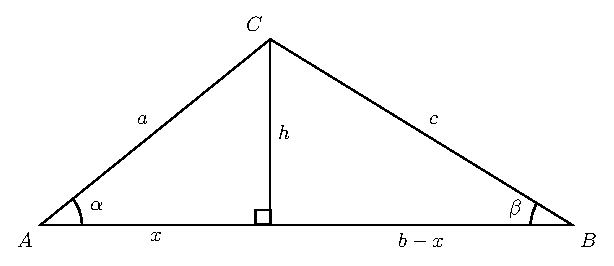
\includegraphics[height=6cm,page=1]{flintprep-triangle}}
\end{center}
If we know one height of the triangle, we can calculate two angles and deduce the third:
\begin{align*}
\sin(\alpha) & = \frac{h}{a} \\
 \sin(\beta) & = \frac{h}{c} \\
      \gamma & = 180 - \alpha - \beta
\end{align*}
where $\alpha$ is the angle at vertex $A$, $\beta$ is the angle at vertex $B$, and $\gamma$ is the angle at vertex $C$ (not shown), with the given distances $AC=a=5$, $AB=b=9$, $BC=c=6$.

To calculate the height, apply the Pythagoras theorem to each half right-triangle:
\begin{align*}
h^2 + x^2 & = a^2 \\
h^2 + (b-x)^2 & = c^2
\end{align*}
Subtract the second equation from the first to eliminate $h^2$, and solve for $x$:
\begin{align*}
(b-x)^2 - x^2 =
b^2 - 2bx = c^2 - a^2 
\quad\Rightarrow\quad
x = \frac{a^2+b^2-c^2}{2b}
\end{align*}
Substitute back to solve for $h$:
\begin{align*}
     h & = \sqrt{a^2-x^2} = \sqrt{a^2 - \left(\frac{a^2+b^2-c^2}{2b}\right)^2}
         \quad \approx 3.142696805 \\
   h/a & \approx 0.628539361 
  \quad\Rightarrow\quad
  \alpha \approx 38.94^{\circ}, \quad 
   \beta \approx 20.44^{\circ}, \quad
  \gamma \approx 120.62^{\circ} 
\end{align*}

\begin{empheq}[box={\mathbox[colback=white]}]{equation*}
 38.94^{\circ} \quad 20.44^{\circ} \quad 120.62^{\circ} 
\end{empheq} 

A general formula for the area of the triangle in terms of the side lengths follows:
\begin{align*}
\frac{bh}{2} 
= \frac{1}{4} \sqrt{(2ab)^2 - \left(a^2+b^2-c^2\right)^2}
\quad \approx 14.14213562
\end{align*}
%% a = 5
%% b = 9
%% c = 6
%% 1/4 * sqrt( (2*a*b)^2 - (a^2+b^2-c^2)^2 )
%% 14.14214
\end{answer}
%%%%%%%%%%%%%%%%%%%%%%%%%%%%%%%%%%%%%%%%%%%%%%%%%%%%%%%%%%%%%%%%%%%%%%%%

\iftoggle{showAnswers}{\newpage}

\end{document}
